\section{Single-task replication}
\label{sec:replication}

We first replicate the single-task addition baseline of
\citet{nanda2023progress} as a validity check, and run the same training
recipe on subtraction and multiplication for later comparison with the
multi-task experiments.

\subsection{Addition baseline}

Figure \ref{fig:fig1_replication} shows the train and test loss curves
for $(a + b) \bmod 113$ with the recipe of Section \ref{sec:methods}.
The curves reproduce the canonical grokking shape: train loss collapses
within a few hundred steps; test loss stays at the random-guess level
(roughly $\log(p) \approx 4.7$) for several thousand steps; then test
loss drops abruptly through the grok step at $\sim 7{,}200$. The
grok step --- the first step at which test accuracy exceeds 0.95 ---
is reported in Table \ref{tab:grok_steps_single}.

\begin{figure}[t]
\centering
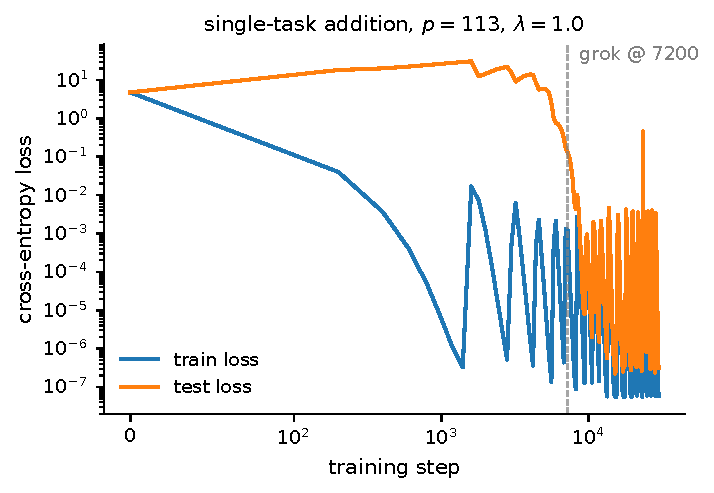
\includegraphics[width=0.85\textwidth]{figures/fig1_replication.pdf}
\caption{Single-task addition replication. Train (blue) and test (orange)
loss for $(a + b) \bmod 113$, $\mathrm{train\_frac} = 0.30$, AdamW with
$\lambda = 1.0$. The training loss collapses within a few hundred steps;
the test loss stays at the random-guess level for $\sim$\textsc{see-log}
steps before grokking. This reproduces Figure 1 of
\citet{nanda2023progress} qualitatively.}
\label{fig:fig1_replication}
\end{figure}

\subsection{Subtraction and multiplication baselines}

Subtraction is a group operation on the same additive group $\Z/p\Z$ as
addition, so we expect quantitatively similar dynamics. Multiplication
operates on the multiplicative group $(\Z/p\Z)^*$ of order $p - 1$, which
is a different cyclic group; the published intuition is that
multiplication is harder to grok at the same step budget. We confirm this
in Figure \ref{fig:fig2_per_op_baselines}.

\begin{figure}[t]
\centering
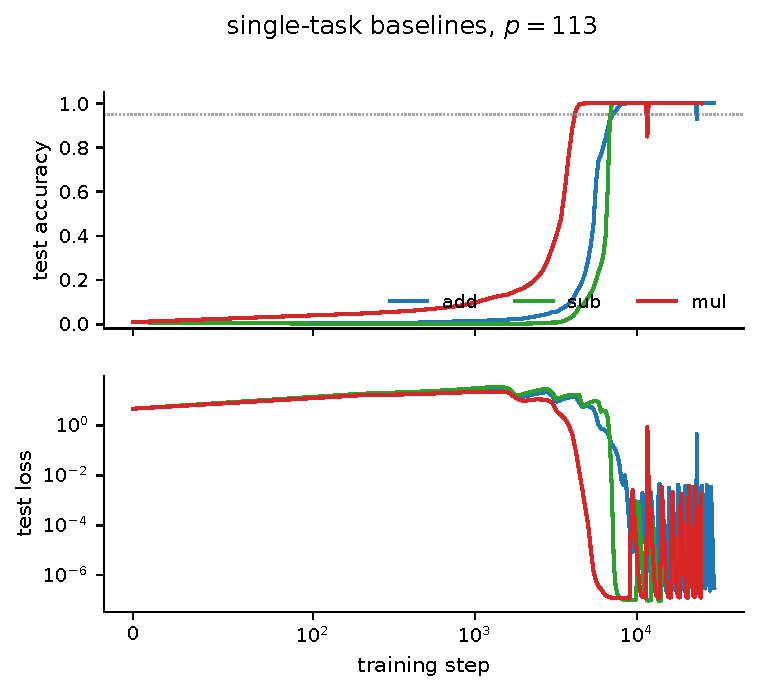
\includegraphics[width=0.95\textwidth]{figures/fig2_per_op_baselines.pdf}
\caption{Single-task baselines on the three operations at $p = 113$.
Test accuracy (\emph{top}) and test loss (\emph{bottom}) are plotted on
a shared $\log$-scaled $x$-axis. Addition and subtraction grok at
similar step counts; multiplication needs a longer schedule.}
\label{fig:fig2_per_op_baselines}
\end{figure}

\begin{table}[t]
\centering
\caption{Single-task grok steps. The grok step is the first step at
which test accuracy exceeds 0.95. ``--'' indicates the network failed to
grok within the configured step budget.}
\label{tab:grok_steps_single}
\begin{tabular}{lr}\toprule\\(awaiting data) & --\\\bottomrule\end{tabular}

\end{table}
